\documentclass[a4paper, 11pt]{article}

%MATH package
\usepackage{amssymb}
\usepackage{amsthm}
\usepackage{amsmath}
%graph package
\usepackage{graphicx}
%table package
\usepackage{booktabs}
%Set FONT
%\usepackage{fontspec}
\topmargin -10mm
\oddsidemargin 0mm
\evensidemargin 0mm
\textwidth 158mm
\textheight 226mm
\parskip 0mm

%title
\title{Progress Report}
\author{Kan Shi}
%date, if blank no date will be displayed
\date{October 2013}

%page number format
\pagenumbering{arabic}

%\setmainfont{Times New Roman}

%Observations
\newtheorem{Ob}{\hskip\parindent\bf{Observation}}[]

\begin{document}
%Generate Title
\maketitle
\vspace{-10mm}

\section{Design of Digit-parallel On-line Multiplier}
\begin{eqnarray}\label{Eq:OnlineMult}
  \left\{\begin{matrix}
    H[j] & = & 2^{-3}(x_{j+4}\cdot Y[j+1]+y_{j+4}\cdot X[j])\\
    W[j] & = & 2P[j]+H[j]\\
    z_j  & = & SEL(\widehat{W[j]})\\
    P[j+1] & = & W[j]-z_j
  \end{matrix}\right.
\end{eqnarray}

%--------------------------------------------------------------------------------------------------
%--------------------------------------------------------------------------------------------------

\section{Probabilistic Model of Overclocking Error in On-line Multiplier}
%In a digit-parallel on-line multiplier, delay can be derived from many sources such as
%For ease of discussion, we
\subsection{Annihilation of the Propagation Chain}\label{subSec:AnnihilationOfChain}

While the delay in a digit-parallel on-line multiplier might be derived from many sources such as the computation delay to generate outputs, the overall delay will eventually be determined by the longest propagation delay between stages with increasing operand word-lengths. Let the propagation delay between two adjacent stages in a $N$-digit olMult be dented by $\mu$, hence the delay of the longest chain which propagates from the MSD to the LSD is given by $d_w$ as shown in~(\ref{Eq:WorstCaseDelay_NaiveAnalysis}).
\begin{eqnarray}\label{Eq:WorstCaseDelay_NaiveAnalysis}
  d_w = (N+\delta-1)\cdot \mu
\end{eqnarray}

However, we note that the chain is annihilated at a certain stage if the propagation inputs of this stage change while the propagation outputs keep stable. This will shrink the value of $d_w$, and there are two possible cases specifically. As an example for the first case, assume at time $t~(t>\mu)$ the value of propagation inputs and outputs of a stage $S_i$ to be $Pin(t)$ and $Pout(t)$ respectively. After delay $\mu$, the input value changes to $Pin(t+\mu)$ and stabilizes thereafter, while the output of this stage remains $Pout(t)$. Hence for the next stage $S_{i+1}$, the input of which varies from $Pout(t-\mu)$ to $Pout(t)$, as illustrated in Figure.xxx. Under this situation, the chain delay to $S_{i+1}$ is reduced by $\mu$ because of the annihilation.
%
\begin{figure}[htbp]
  \centering
  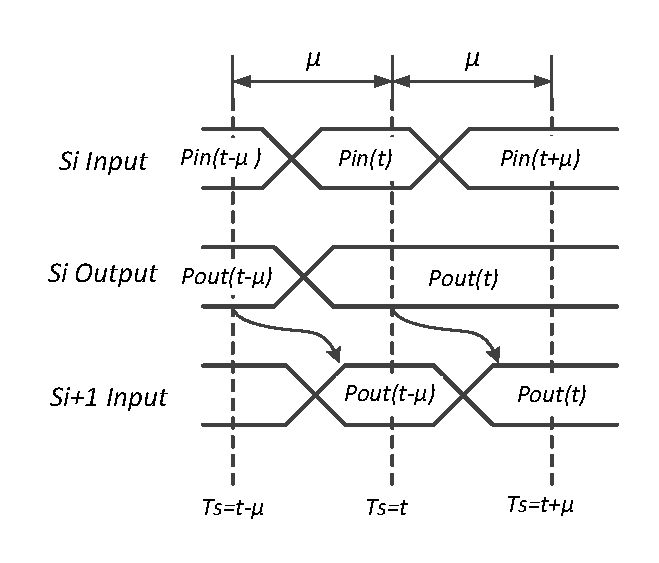
\includegraphics[width=.5\textwidth]{./Figures/TimingWave.pdf}
  \caption{Timing wave.}
\end{figure}

For the second case, the current chain will be completely annihilated and a new chain will be generated at a given stage if $Pout(t)=Pout(0)$ for $t=\mu,~2\mu,~\cdots$. Therefore the worst case delay is given by~(\ref{Eq:OverallPathDelay_MultiPaths}) where $d_p$ denotes the delay of the $p^{th}$ propagation chain.
\begin{eqnarray}\label{Eq:OverallPathDelay_MultiPaths}
  d_w'=max(d_1,~d_2,~\cdots)
\end{eqnarray}

In the following of this section, detailed analysis for both cases will be described and the worst-case delay of the olMult will be discussed.
%--------------------------------------------------------------------------------------------------

\subsection{Worst-case Analysis in On-line Multiplier}
\subsubsection{Two Observations}
From (\ref{Eq:OnlineMult}) two observations can be made under the assumption that all signals are reset to $0$ initially.

%\newtheorem{Ob}{Observation}\label{Ob:Ob1}
\begin{Ob}\label{Ob:Ob1}
    The two integer bits of $W[j]$ and $2P[j+1]$ are either $00$ or $11$.
\end{Ob}

This observation can be justified by contradiction. All the combinations of $\widehat{W[j]}$ and the corresponding $z_j$, the most significant 3 bits of $P[j+1]$ and the 2 integer bits of $2P[j+1]$ are listed in Table~\ref{Tab:Observation1}. For $j=-3$, we have (\ref{Eq:olMult_Stage0}) according to (\ref{Eq:OnlineMult}).
\begin{eqnarray}\label{Eq:olMult_Stage0}
\left\{\begin{matrix}
    W[-3] & = & 2^{-3}(y_1\cdot X[-3])\\
    H[-2] & = & W[-3]
\end{matrix}\right.
\end{eqnarray}

Hence $\widehat{W[-3]}$ is either $11.1$ or $00.0$, with the corresponding $2P[-2]$ being $00$ or $11$ which is the propagation input for the next stage. For $j>-3$, the 3 MSBs of $H[j]$ in (\ref{Eq:OnlineMult}) is either $00.0$ or $11.1$ due to the shift of binary point. Also as seen in Table.xxx, if the two integer bits of $\widehat{W[j]}$ are identical, the integer bits of $2P[j+1]$ will be the same. Therefore the propagation of $2P[j+1]$ will not generate diverse bits in the integer part of $W[j]$.
%
\begin{table}[htbp]
\caption{All the combinations of $\widehat{W[j]}$ and the corresponding $z_j$, $P[j+1]$ and $2P[j+1]$.}
\centering
%\vspace{10ex}
\begin{tabular}{c|ccc}
\toprule
 $\widehat{W[j]}$ & $z_j$ & $P[j+1]$ (3 MSBs)  & $2P[j+1]$ (2 MSBs) \\ \midrule
 $00.0$ & $0$ & $00.0$ & $00$\\
 $00.1$ & $1$ & $11.1$ & $11$\\
 $01.0$ & $1$ & $00.0$ & $00$\\
 $01.1$ & $1$ & $00.1$ & $01$\\
 $10.0$ & $\bar{1}$ & $11.0$ & $10$\\
 $10.1$ & $\bar{1}$ & $11.1$ & $11$\\
 $11.0$ & $\bar{1}$ & $00.0$ & $00$\\
 $11.1$ & $0$ & $11.1$ & $11$\\ \bottomrule
\end{tabular}
\label{Tab:Observation1}
\end{table}

\begin{Ob}\label{Ob:Ob2}
    $P[j+1]$ will not change if only the integer bits of $W[j]$ change to a new value.
\end{Ob}

According to Observation~\ref{Ob:Ob1}, there are only four possible cases for the change of $W[j]$ as summarized in Table.xxx. This observation describes the situation where a propagation chain annihilates but not necessarily generating a new chain, because $2P[j+1]$ may not maintain its initial value at all times.
%
\begin{table}[htbp]
\caption{Ob2.}
\centering
\begin{tabular}{c|ccc}
\toprule
 $\widehat{W[j]}$ & $z_j$ & $P[j+1]$ (3 MSBs)  & $2P[j+1]$ (2 MSBs) \\ \midrule
 $00.0\rightarrow11.0$ & $0\rightarrow\bar{1}$ & $00.0$ & $00$\\
 $00.1\rightarrow11.1$ & $1\rightarrow\bar{0}$ & $11.1$ & $11$\\
 $11.0\rightarrow00.0$ & $\bar{1}\rightarrow0$ & $00.0$ & $00$\\
 $11.1\rightarrow00.1$ & $0\rightarrow{1}$ & $11.1$ & $11$\\ \bottomrule
\end{tabular}
\label{Tab:Observation2}
\end{table}

% only result in $11.1$ or $00.0$ for the most significant 3 bits of $W[j]$. In addition for $2P[j+1]$, there are only two cases ($01$ and $10$) violate Observation~\ref{Tab:Observation1}. The corresponding value of $\widehat{W[j]}$ are $01.1$ and $10.0$ respectively.
\subsubsection{Annihilation of the Propagation Chain in An olMult }
As stated in Section~\ref{subSec:AnnihilationOfChain}, the annihilation of propagation chain would leads to a reduction of the propagation delay. It is worthwhile exploring the conditions of occurrence of Observation~\ref{Ob:Ob2}. For instance in a 3-digit olMult, there are 6 stages in total, as shown in Fig.xxx. If $x_{-3}\neq0$ and/or $y_{-3}\neq0$, no more than 6 MSBs of $P[-2]$ will change with respect to the initial value at $t=0$. This is because in (\ref{Eq:olMult_Stage0}) $y_1\cdot X[-3]$ contains only 1 fractional bit and 2 integer bits. Hence maximally 5 MSBs of $2P_{[-2]}(0)$ will be updated and thereafter stabilized. It is worth noting that this is irrelevant to the word-length of the olMult. Additionally as assumed previously in the timing model, at $t=0$ the computation of $H[j]~(j\in[-2,2])$ in (\ref{Eq:OnlineMult}) is finished. This results in $2P_{[j]}(0)$, which will be updated sequentially with a delay of $\mu$, triggered by the propagation of $2P_{[-2]}(0)$. During each propagation, the number of the altered MSBs will be reduced by 1, because of the shifting of the binary point in $2P[j]$. For example, $2P_{[-1]}(t)$ stabilizes when $t=\mu$, and the altered MSBs for $2P_{[-1]}(0)\rightarrow2P_{[-1]}(\mu)$ are 4 bits. This process repeats until $S_1$, of which the changed MSBs for $2P_{[1]}(3\mu)\rightarrow2P_{[1]}(4\mu)$ are 2 bits. According to Observation~\ref{Ob:Ob2}, the chain triggered by $2P_{[-2]}(0)$ is annihilated at $S_1$. Therefore the propagation delay from $S_{-3}$ to $S_2$ is $4\mu$.
 
%$ For $t>0$, the variation of $2P[j]$ propagates from $S_{-3}$ to $S_{-2}\cdots S_1$ with the number of altered MSBs being $5\cdots2$, from $t=\mu$ to $t=4\mu$ respectively. Also note that this changing procedure is irrelevant to the value of $x_{j+4}$, $y_{j+4}$, $X[j]$ and $Y[j+1]$ for $S_{-2}\cdots S_1$. Hence for $2P_{[1]}(3\mu)\rightarrow2P_{[1]}(4\mu)$, we have $2P_{[2]}(3\mu)=2P_{[2]}(4\mu)$ in accordance with Observation~\ref{Ob:Ob2}. This stands for an annihilation of the chain, and therefore the propagation delay from $S_{-3}$ to $S_2$ is $4\mu$.

\begin{figure}[htbp]
  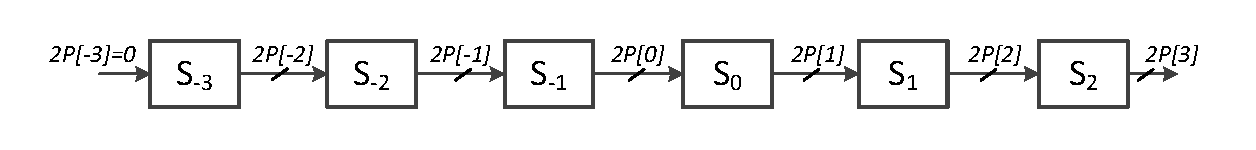
\includegraphics[width=\textwidth]{./Figures/OlMult_Stage.pdf}
  \caption{Propagation chain in 3-digit olMult}
\end{figure}

It is worth noting that in this example, the chain still propagates through $S_2$ without generating a new chain. Because it is hardly to achieve $2P_{[2]}(t)\equiv2P_{[2]}(0)$ with $t=\mu,~2\mu,\cdots$, due to the propagation of $2P_{[j]}(t)$ where $j\in[-2,1]$. The maximum number of the changed MSBs for $2P_{[2]}(3\mu)\rightarrow2P_{[2]}(4\mu)$ is 3, because this is actually triggered by $2P_{[-1]}(0)$, which varies 6 MSBs in comparison to its initial value. Likewise there will be maximally 4 MSBs changing for $2P_{[3]}(4\mu)\rightarrow2P_{[3]}(5\mu)$.

The above changing process happens in a 3-digit olMult when $P[-2]\neq0$, which is only determined by the inputs of the first stage regardless of the other stages. Actually in other situations, the overall propagation delay will not be increased. For example for $t=0,~\mu,~\cdots$ if $P_{[-2]}(t)=0$ while $P_{[-1]}(t)\neq0$, the chain starts from $2P_{[-1]}(0)$. Based on a similar analysis, the chain will finally annihilate at $S_2$, of which we have 2 MSBs changing for $2P_{[2]}(3\mu)\rightarrow2P_{[2]}(4\mu)$, yielding a delay of $4\mu$. This value shrinks to $3\mu$ if $P_{[-2]}(t)=P_{[-1]}(t)=0$ while $P_{[0]}(t)\neq0$ for $t=0,~\mu,~\cdots$.

\subsubsection{State Transition Graph in An olMult}
For an olMult with a greater word-length, the aforementioned process is still valid. Annihilation happens at $S_i$ when there are only 2 MSBs of $2P_{[i]}(t)$ update before it is stabilized. Otherwise the propagation continues regardless of the inputs $x_{j+4},~y_{j+4},~X[j]$ and $Y[j+1]$ of $S_j$. The propagation process from $S_1$ can be illustrated using a state transition graph. One possible transition path from $S_1$ in a 5-digit olMult is shown in Fig.xxx, where a state $S_{mn}$ denotes the propagation input of $Stage~m$ changes $n$ MSBs prior to stabilization. The transition probabilities are labelled on the edges. For instance $P_{12\_23}$ denotes the conditional probability $P(S_{23}\mid S_{12})$. Note that $P_{23\_32}=1$ because annihilation only happens when $n=2$ in $S_{mn}$. In this case, the probability of this transition path is given by~(\ref{Eq:TransitionProb_OnePath}), where $P(S_{12})$ is determined by the value of $x_1$ and $y_1$ because $S_{12}$ will happen when $2P_{[-2]}(0)\neq0$.
\begin{eqnarray}\label{Eq:TransitionProb_OnePath}
\begin{split}
  P_{trans} &= P(S_{42},~S_{32},~S_{23},~S_{12})\\
            &= P(S_{42}\mid S_{32},~S_{23},~S_{12})P(S_{32}\mid S_{23},~S_{12})P(S_{23}\mid S_{12})P(S_{12})\\
            &= P_{32\_42}\cdot1\cdot P_{12\_23}\cdot P(S_{12}) 
\end{split}
\end{eqnarray}

The delay of this transition path can also be determined by counting the number of states $S_{m2}$. First, there is no annihilation prior to $S_{12}$. Second, $S_{42}$ is excluded because it is not necessary to wait for the propagation output of this stage to generate before sampling $z_4$. Hence there are totally 2 annihilation states $S_{12}$ and $S_{32}$ in this path. According to (\ref{Eq:WorstCaseDelay_NaiveAnalysis}) the worst case delay without any annihilation is $d_w=7\mu$. Delay of a specific transition path is given by (\ref{Eq:Delay_TransitionPath}). Hence the delay of this path is $5\mu$.
%
\begin{eqnarray}\label{Eq:Delay_TransitionPath}
  d = d_w - \mu\cdot AnnihilationNo.  
\end{eqnarray}

Additionally as discussed earlier, there are other possible states when annihilation happens. The complete transition graph of a 5-digit olMult is shown in Fig.xxx.



% transition graph 
 
 %In the previous example where $P[-2]\neq0$, there is no new chain generated. Instead, the chain propagates to $S_2$, because $2P_{[-1]}(t)\cdots 2P_{[2]}(t)$ will prevent $2P_{[3]}(t)$ maintaining its initial value before $2P_{[-2]}(0)$ propagates down to $S_2$. In this case, the propagation input of $S_2$ changes from $2P_{[2]}(3\mu)$ to $2P_{[2]}(4\mu)$ and stabilizes, as illustrated in Fig.xxx(previous figure).

%the temporal results of $S_{1}\cdots S_{-2}$, i.e. $P[2]\cdots P[-1]$, will prevent $P[3]$ maintaining the initial value before $2P[-2]$ propagates down to $S_2$. 

%, with the maximum number of changed MSBs being $3$. Similarly, if $3$ MSBs are changing from $2P_{[2]}(3\mu)$ to $2P_{[2]}(4\mu)$, there will be $2$ MSBs that
%
%However the number of bits that change in MSBs would be different.
%
%As an example for $S_5$, there are maximally


\subsection{Probability of Overclocking Error in On-line Multiplier}

\subsection{Magnitude of Overclocking Error in On-line Multiplier}

%------------------------------------------------------------------------
\section{Probabilistic Model of Truncation Error in On-line Operators}


\end{document} 